% !TEX root = ../notes_template.tex
\chapter{Muscle Excitation}\label{chp:excitation}

% Find and replace
% Na with $Na^+$
% K with $K^+$
% Cl with $Cl^-$
% Ca with $Ca^{2+}$
% H with $H^+$
% Mg with $Mg^2+$


\minitoc

This chapter covers muscle excitation, the molecular mechanisms that allow excitation, and related clinical physiology connections. 

Muscle fiber excitation starts with an excited motor axon ($\alpha$-motor neuron) and ends with the binding of calcium to troponin. Binding calcium to troponin allows a crossbridge to go from an inactivated to an activated state. The final step in muscle excitation is the coupling between excitation and activation (Excitation - Activation Coupling). 

The underlying molecular mechanisms of the muscle excitation pathway are fundamental to many areas of clinical physiology. The mechanisms include the characteristics and actions of excitable membranes. Excitable membrane characteristics include ion channels, pumps and receptors. Actions include using transport to establish a resting membrane potential and the ability to have an action potential (excitation). 

Understanding excitable membranes creates Clinical Physiology Connections opportunities in three areas: 1. system wide regulatory function of the neuroendocrine system; 2. function of sensory receptors; and 3. pharmacodynamics.

\vspace{5mm}

\textbf{Objectives include:}
\begin{enumerate}
    \item Explain the events of muscle excitation and excitation - activation coupling.
    \item Relate the events of excitation - activation coupling to the creation of active tension.
\item Explain the components and capabilities of an excitable membrane.
    \item Explain the events that result in sarcolemma depolarization.
   \item Explain the events that result in neuromuscular endplate depolarization.
    \item Explain the function and role of the neuroendocrine system for homeostasis.
\item Explain the basic function of sensory receptors.
    \item Explain pharmacodynamics based on actions occurring at end organ receptors
   \item Demonstrate the ability to apply basic physiology concepts such as the cell membrane, mass balance, and flow gradients to the analysis of patient/client problems related to the generation of muscle excitation, the effectiveness of the neuroendocrine system and pharmaceuticals.
\end{enumerate}

\section{Muscle Fiber Excitation}
\paragraph{Excitation}
% THis section needs work!!!
Muscle fiber excitation is the signal that initiates crossbridge activation and results in a twitch. Excitation is a state of the membrane. Based on the concept of excitation a muscle fiber exists in one of two states, resting or excitation. Excitation occurs when a membrane depolarizes and the process of depolarizing is called an action potential (AP). The resting state of the membrane has is polarized and is called the resting membrane potential. Cellular membranes that can undergo excitation is an excitable membrane, and this includes nerve and muscle cell membranes. 
\paragraph{Excitation as Signal Transduction}
Excitation is a mechanism for signal transduction (sending and receiving signals). One example is when membrane excitation results in an action in the cell that influences cellular processes, which includes processes such as exocytosis,\footnotemark\footnotetext{Exocytosis is a form of active transport and bulk transport in which a cell transports molecules (e.g., neurotransmitters and proteins) out of the cell). From \url{https://en.wikipedia.org/wiki/Ligand}}. A second example is when a membrane is excited through binding of a ligand\footnotemark\footnotetext{A ligand is any molecule or atom which binds reversibly to a protein. A ligand can be an individual atom or ion. It can also be a larger and more complex molecule made from many atoms. A ligand can be natural, as an organic or inorganic molecule. A ligand can also be made synthetically, in the laboratory. From \url{https://biologydictionary.net/ligand/}} to a receptor on its surface which can then excite the surface, direct another signal into the cell (or both). 

\subsection{Muscle Fiber Excitation Overview}
\paragraph{}

Skeletal muscle fiber excitation starts with excitation of an $\alpha$-motor neuron (Step 1 in Figure \ref{fig:excitation_overview}) which crosses the neuromuscular junction (NMJ) and excites the motor end plate (Step 2 in Figure \ref{fig:excitation_overview}). Excitation of the motor end plate causes excitation of the sarcolemma, which causes excitation of the transverse tubule system (T-tubules). Excitation of T-tubules cause excitation of the sarcoplasmic reticulum (SR), which causes the release of calcium into the muscle fiber and the activation of available crossbridges (Step 3 in Figure \ref{fig:excitation_overview}) This last step (Step 3 in Figure \ref{fig:excitation_overview}). Excitation of the SR and release of Ca is referred to as Excitation-Activation Coupling (or Excitation-Contraction Coupling). A single excitation results in a twitch.

% Change this image to include an AP graphic instead of a lightening bolt! 

\begin{figure}[!ht]
    \centering
    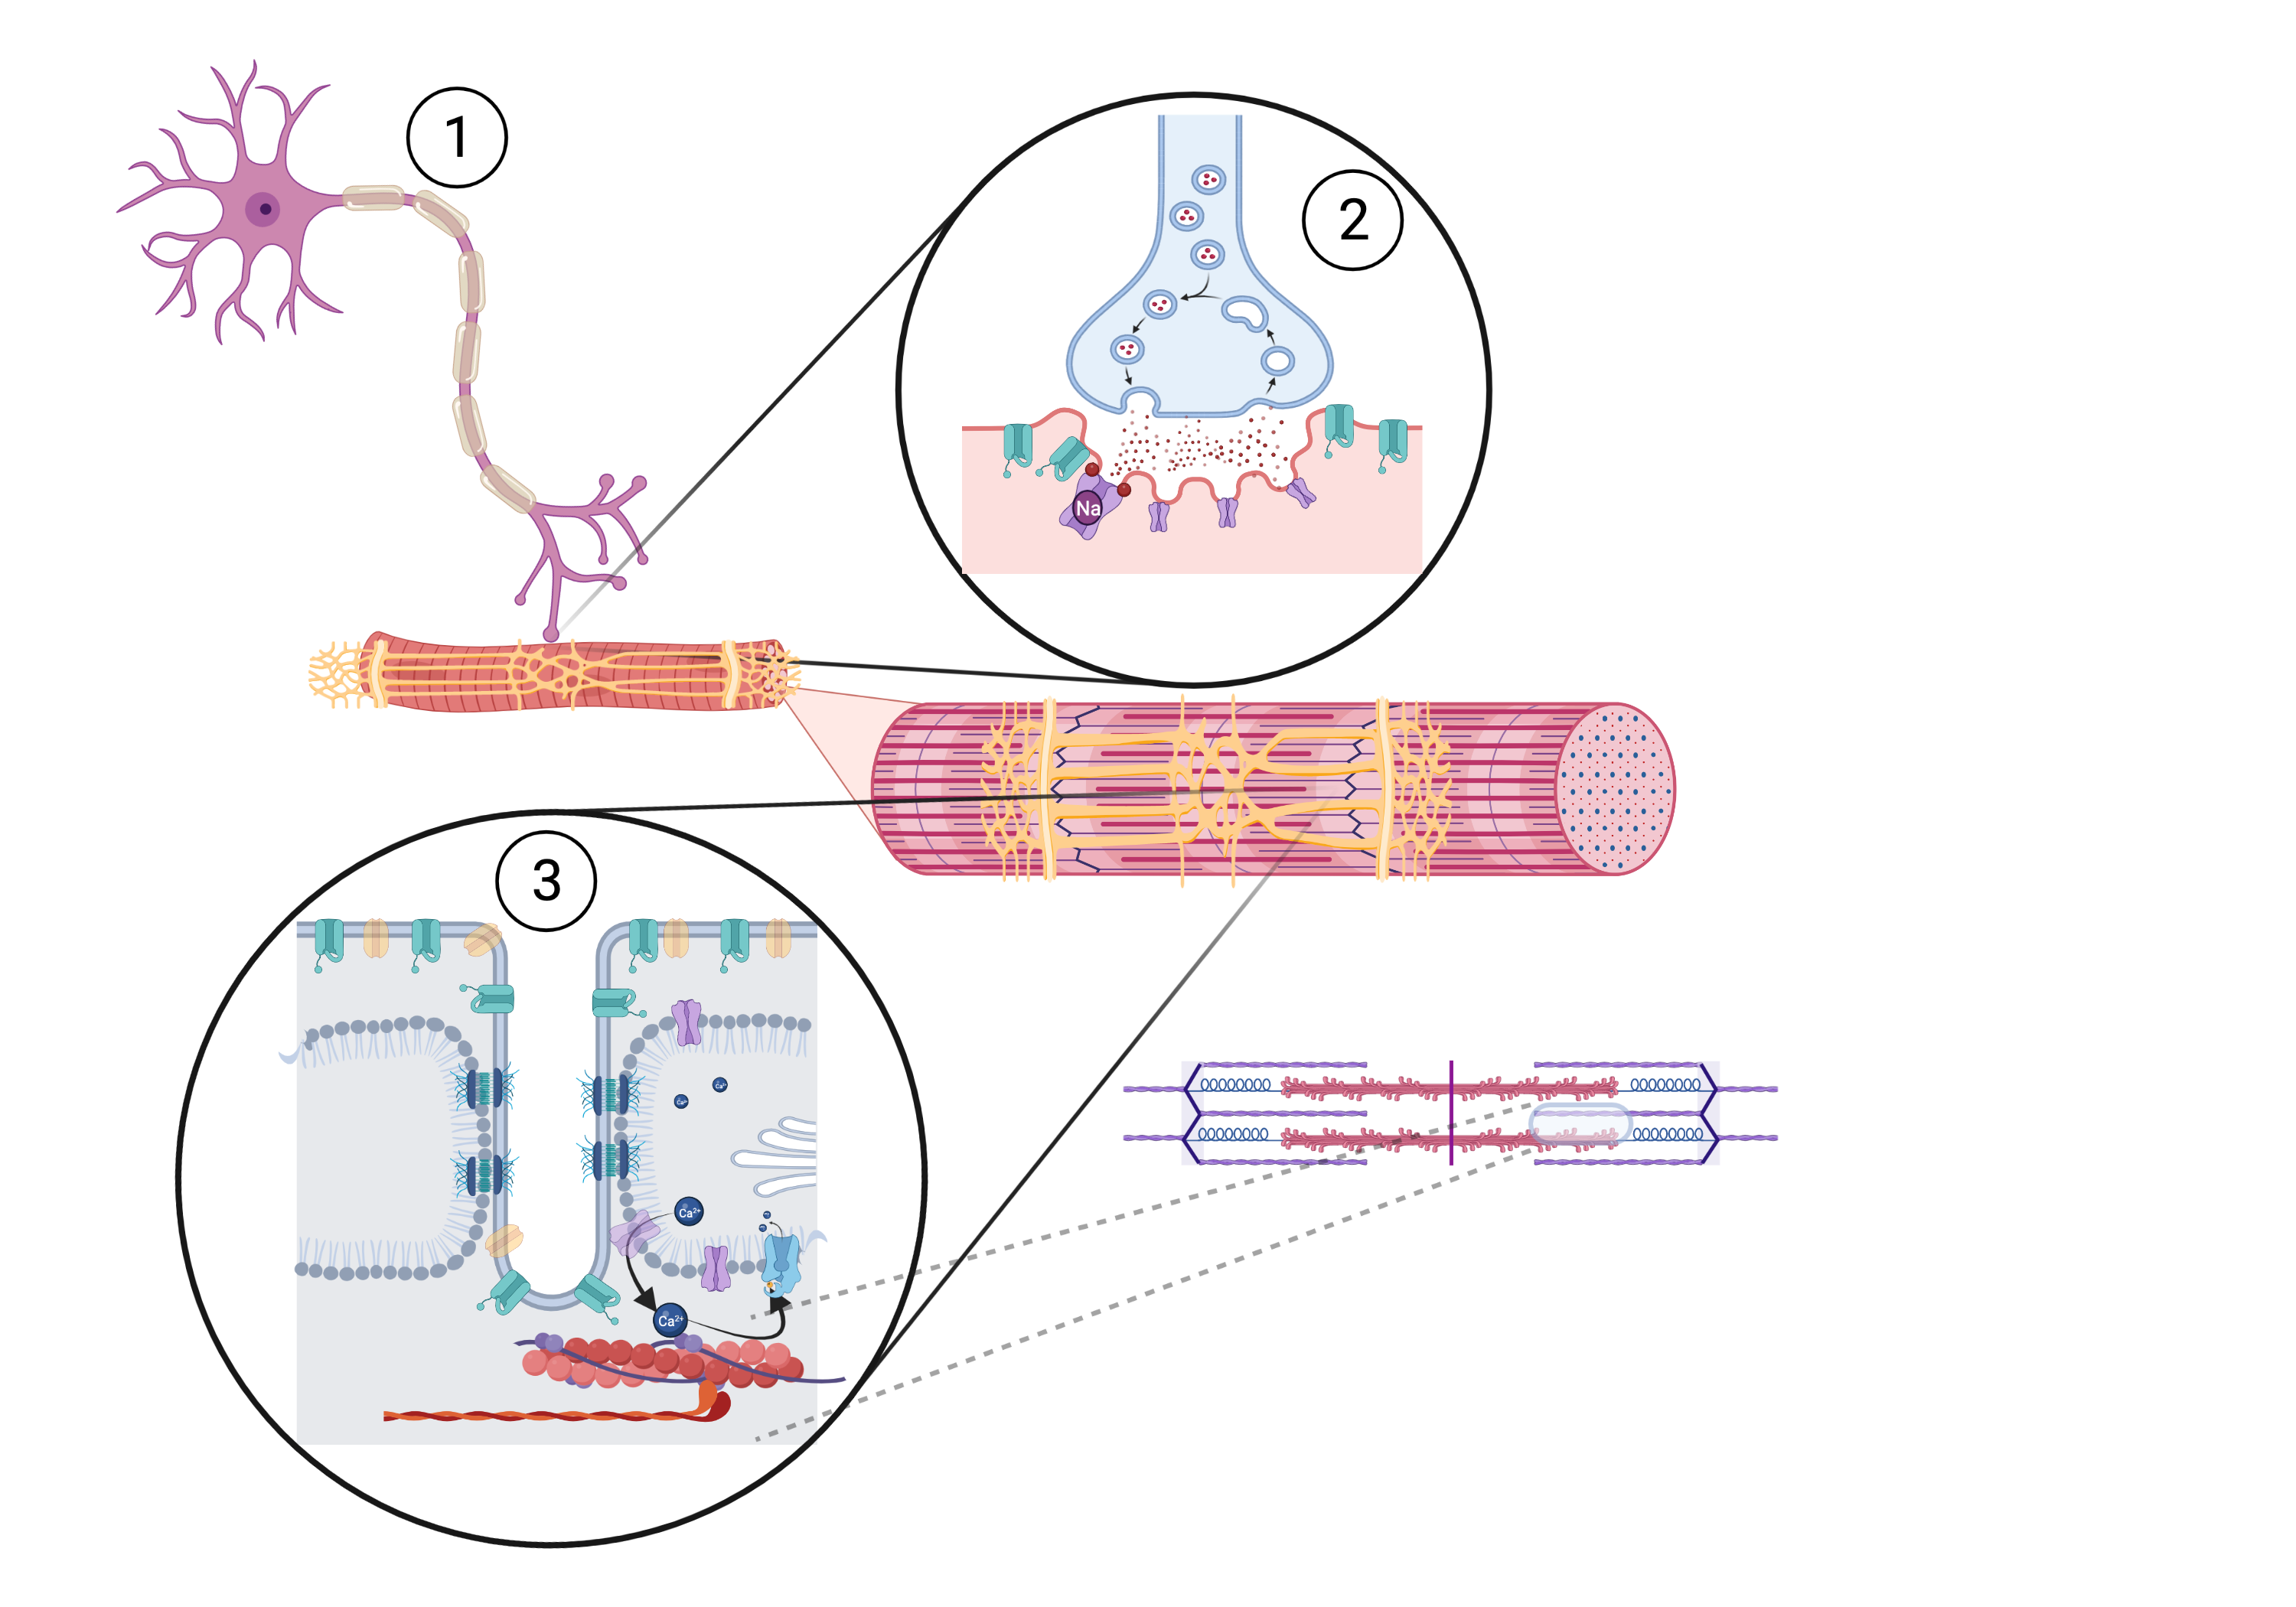
\includegraphics[width=1\linewidth]{./figure/excitation_overview.png}
    \caption{Overview of excitation from the $\alpha$ motor neuron to crossbridge activation \footnotesize{Created with BioRender.com}}
    \label{fig:excitation_overview}
\end{figure}

\subsection{Step 1 - The $\alpha$-Motor Neuron}
Excitation of an $\alpha$-motor neuron is regulated by the central nervous system and occurs at the membrane of its dendrites in the spinal cord. A wave of excitation travels along the axon to its terminal branches at neuromuscular junctions (NMJs) by sequential excitation facilitated by voltage gated ion channels. Each muscle fiber has one NMJ and receives one axon terminal. However, each $\alpha$-motor neuron has a variable number of terminal branches (See Chapter \ref{chp:regulation}.  Excitation travels from the spinal cord to the NMJ by means of saltatory conduction which allows excitation to big steps as it travels along the axon membrane. Saltatory conduction increases the nerve conduction velocity and is made possible by the myelin sheathes (Figure \ref{fig:Motoneuron}). The membrane is exposed along the axon at nodes of Ranvier. Excitation travels by jumping from one node of Ranvier to the next.\footnotemark\footnotetext{The implications of the myelin sheath on nerve conduction velocity is detailed in Chapter \ref{chp:regulation} as an important consideration for muscle tension regulation.} 

\begin{figure}[!ht]
    \centering
    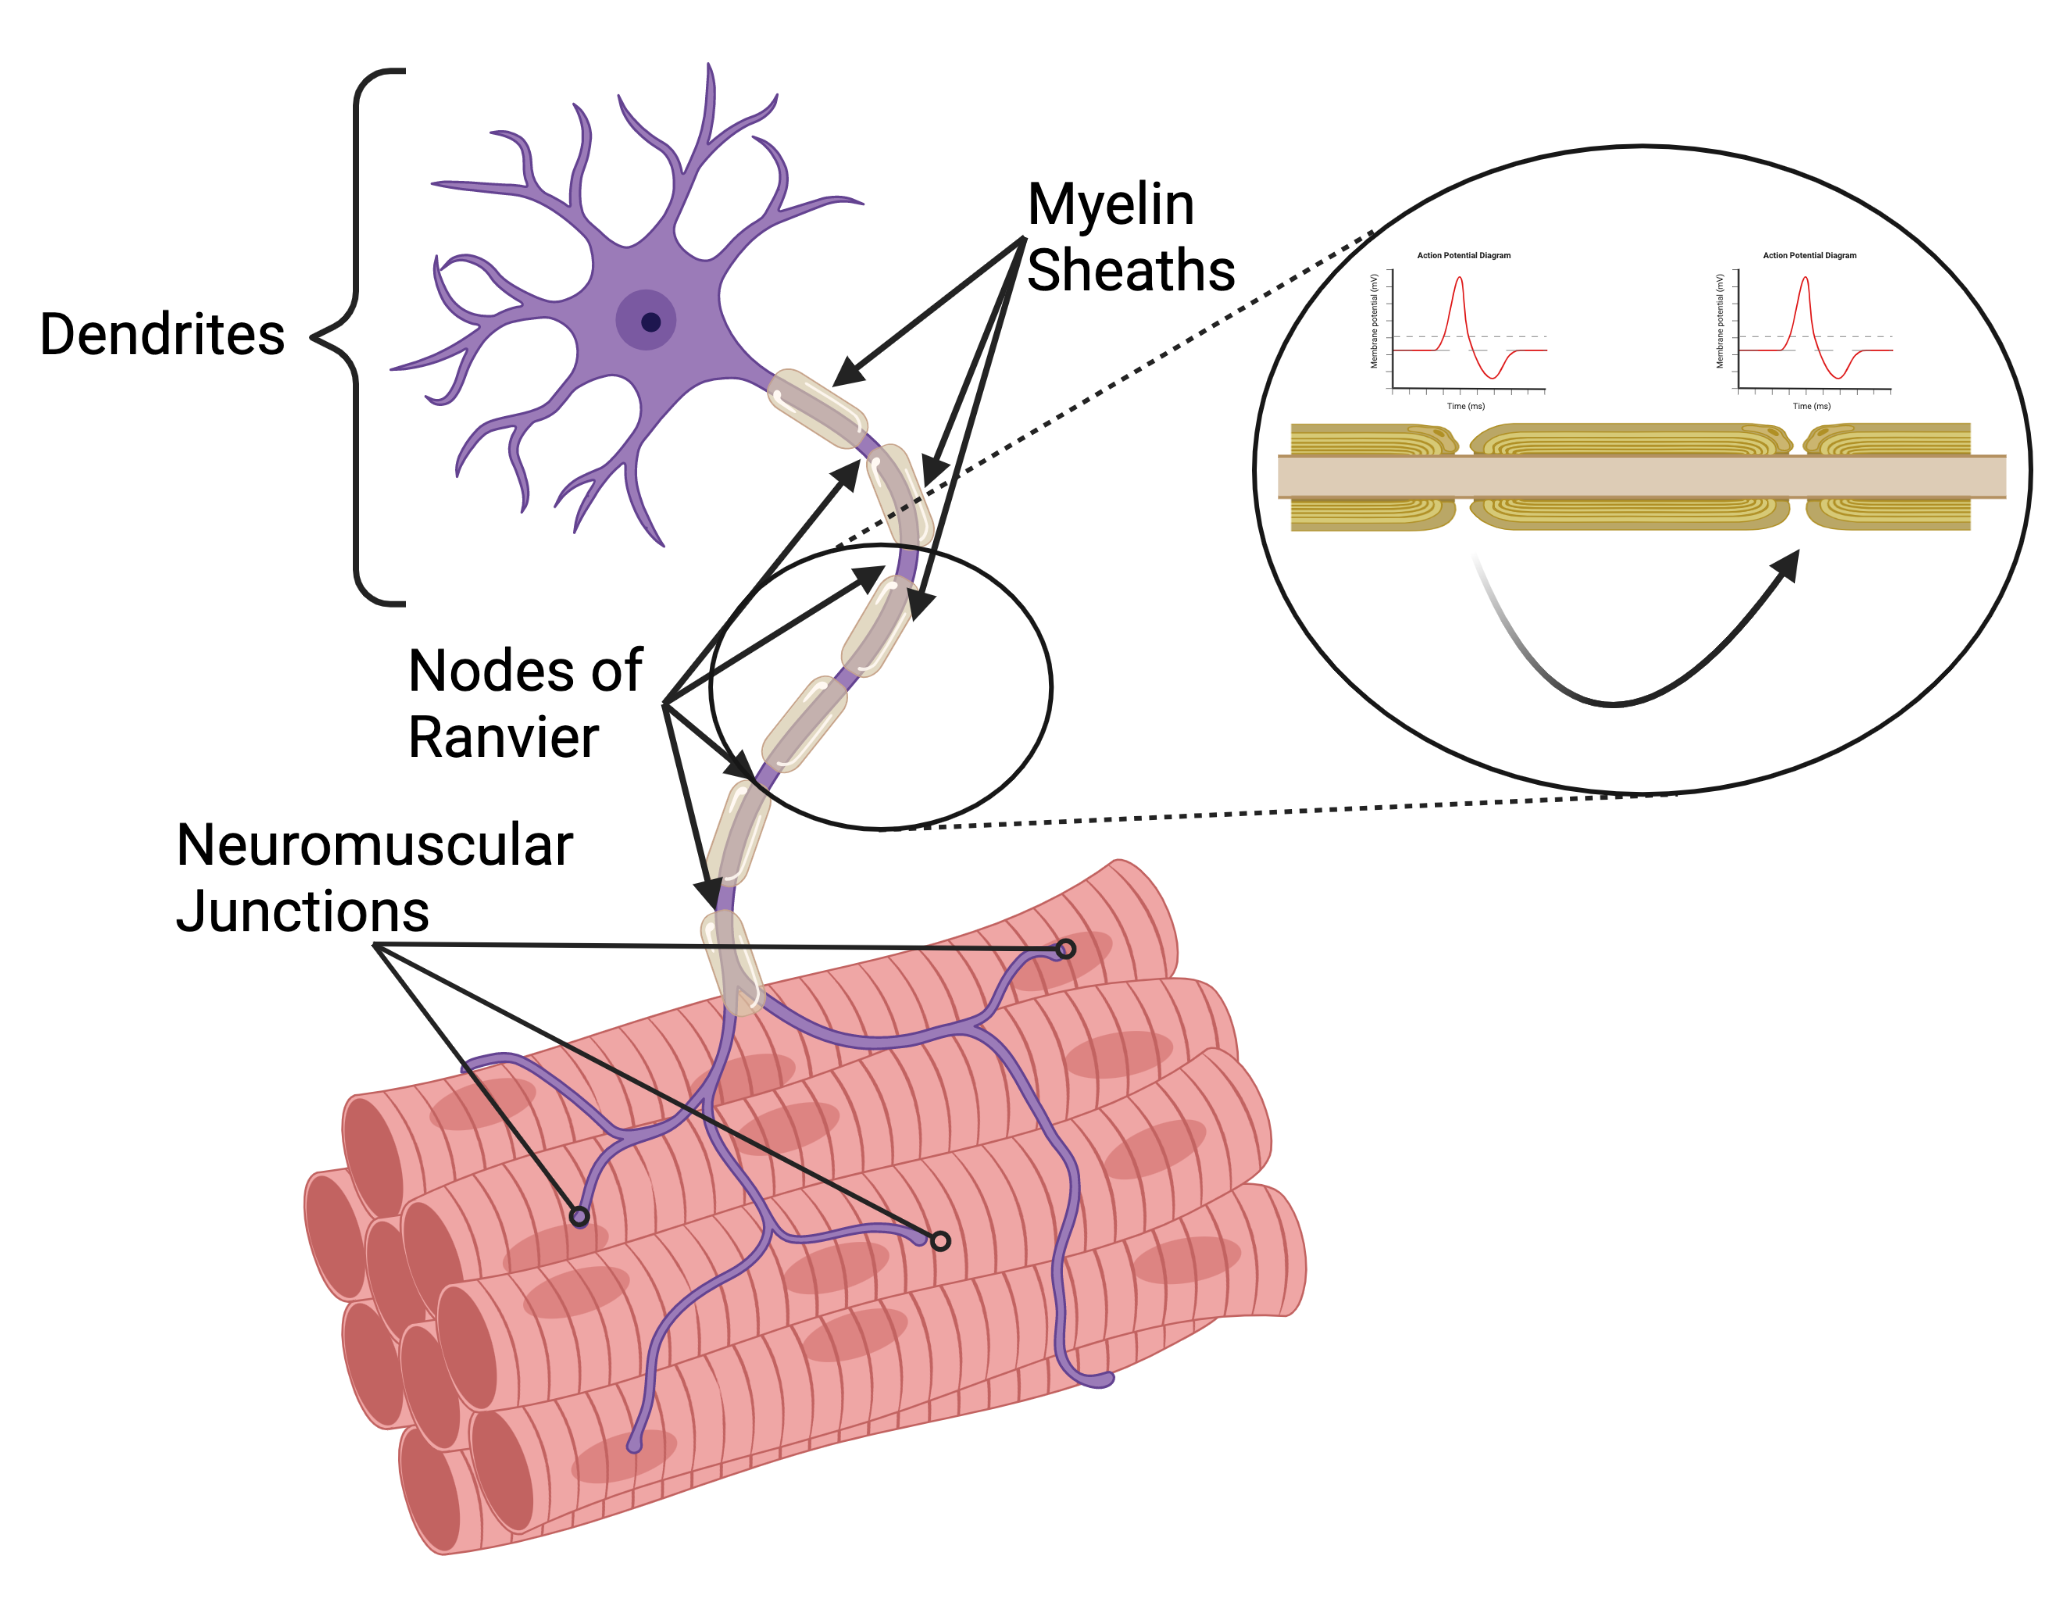
\includegraphics[width=1\linewidth]{./figure/Motoneuron.png}
    \caption{$\alpha$-motor neuron terminating at several muscle fiber motor end plates \footnotesize{Created with BioRender.com}}
    \label{fig:Motoneuron}
\end{figure}

\subsection{Step 2 - Neuromuscular Junction - Motor End Plate - Sarcolemma Excitation}

Membrane excitation at the axon terminal releases the neurotransmitter acetylcholine (ACh) due to the action of voltage gated Ca channels. Interestingly, these channels are inhibited by high magnesium (Mg) concentrations. ACh crosses the NMJ synapse (Figure \ref{fig:NMJ} and excites the motor end plate by binding to receptors and opening ligand gated ion channels. For tight regulation of muscle activation at the NMJ, ACh is quickly broken down by cholinesterase (an enzyme synthesized by the muscle fiber that hydrolyzes ACh) and free choline molecules are transported into the axon terminal (endocytosis) to be resynthesized. However, when high concentrations of ACh accumulate at the NMJ there are two processes that can result in more rapid excitation of the motor end plate. Temporal summation refers to repeated stimulation of one receptor by ACh; and spatial summation refers to stimulation of a larger number of motor end plate receptor. Frequency summation is limited by the amount of ACh, which is influenced by the release of ACh from the axon terminal and the breakdown of ACh in the NMJ. Spatial summation is also limited by the amount of ACh, but it is also limited by the number of receptors on the motor end plate.

%Need to create NMJ - sarcolemma figure - more detail than but based on Step 2 in overview figure

\begin{figure}[!ht]
    \centering
    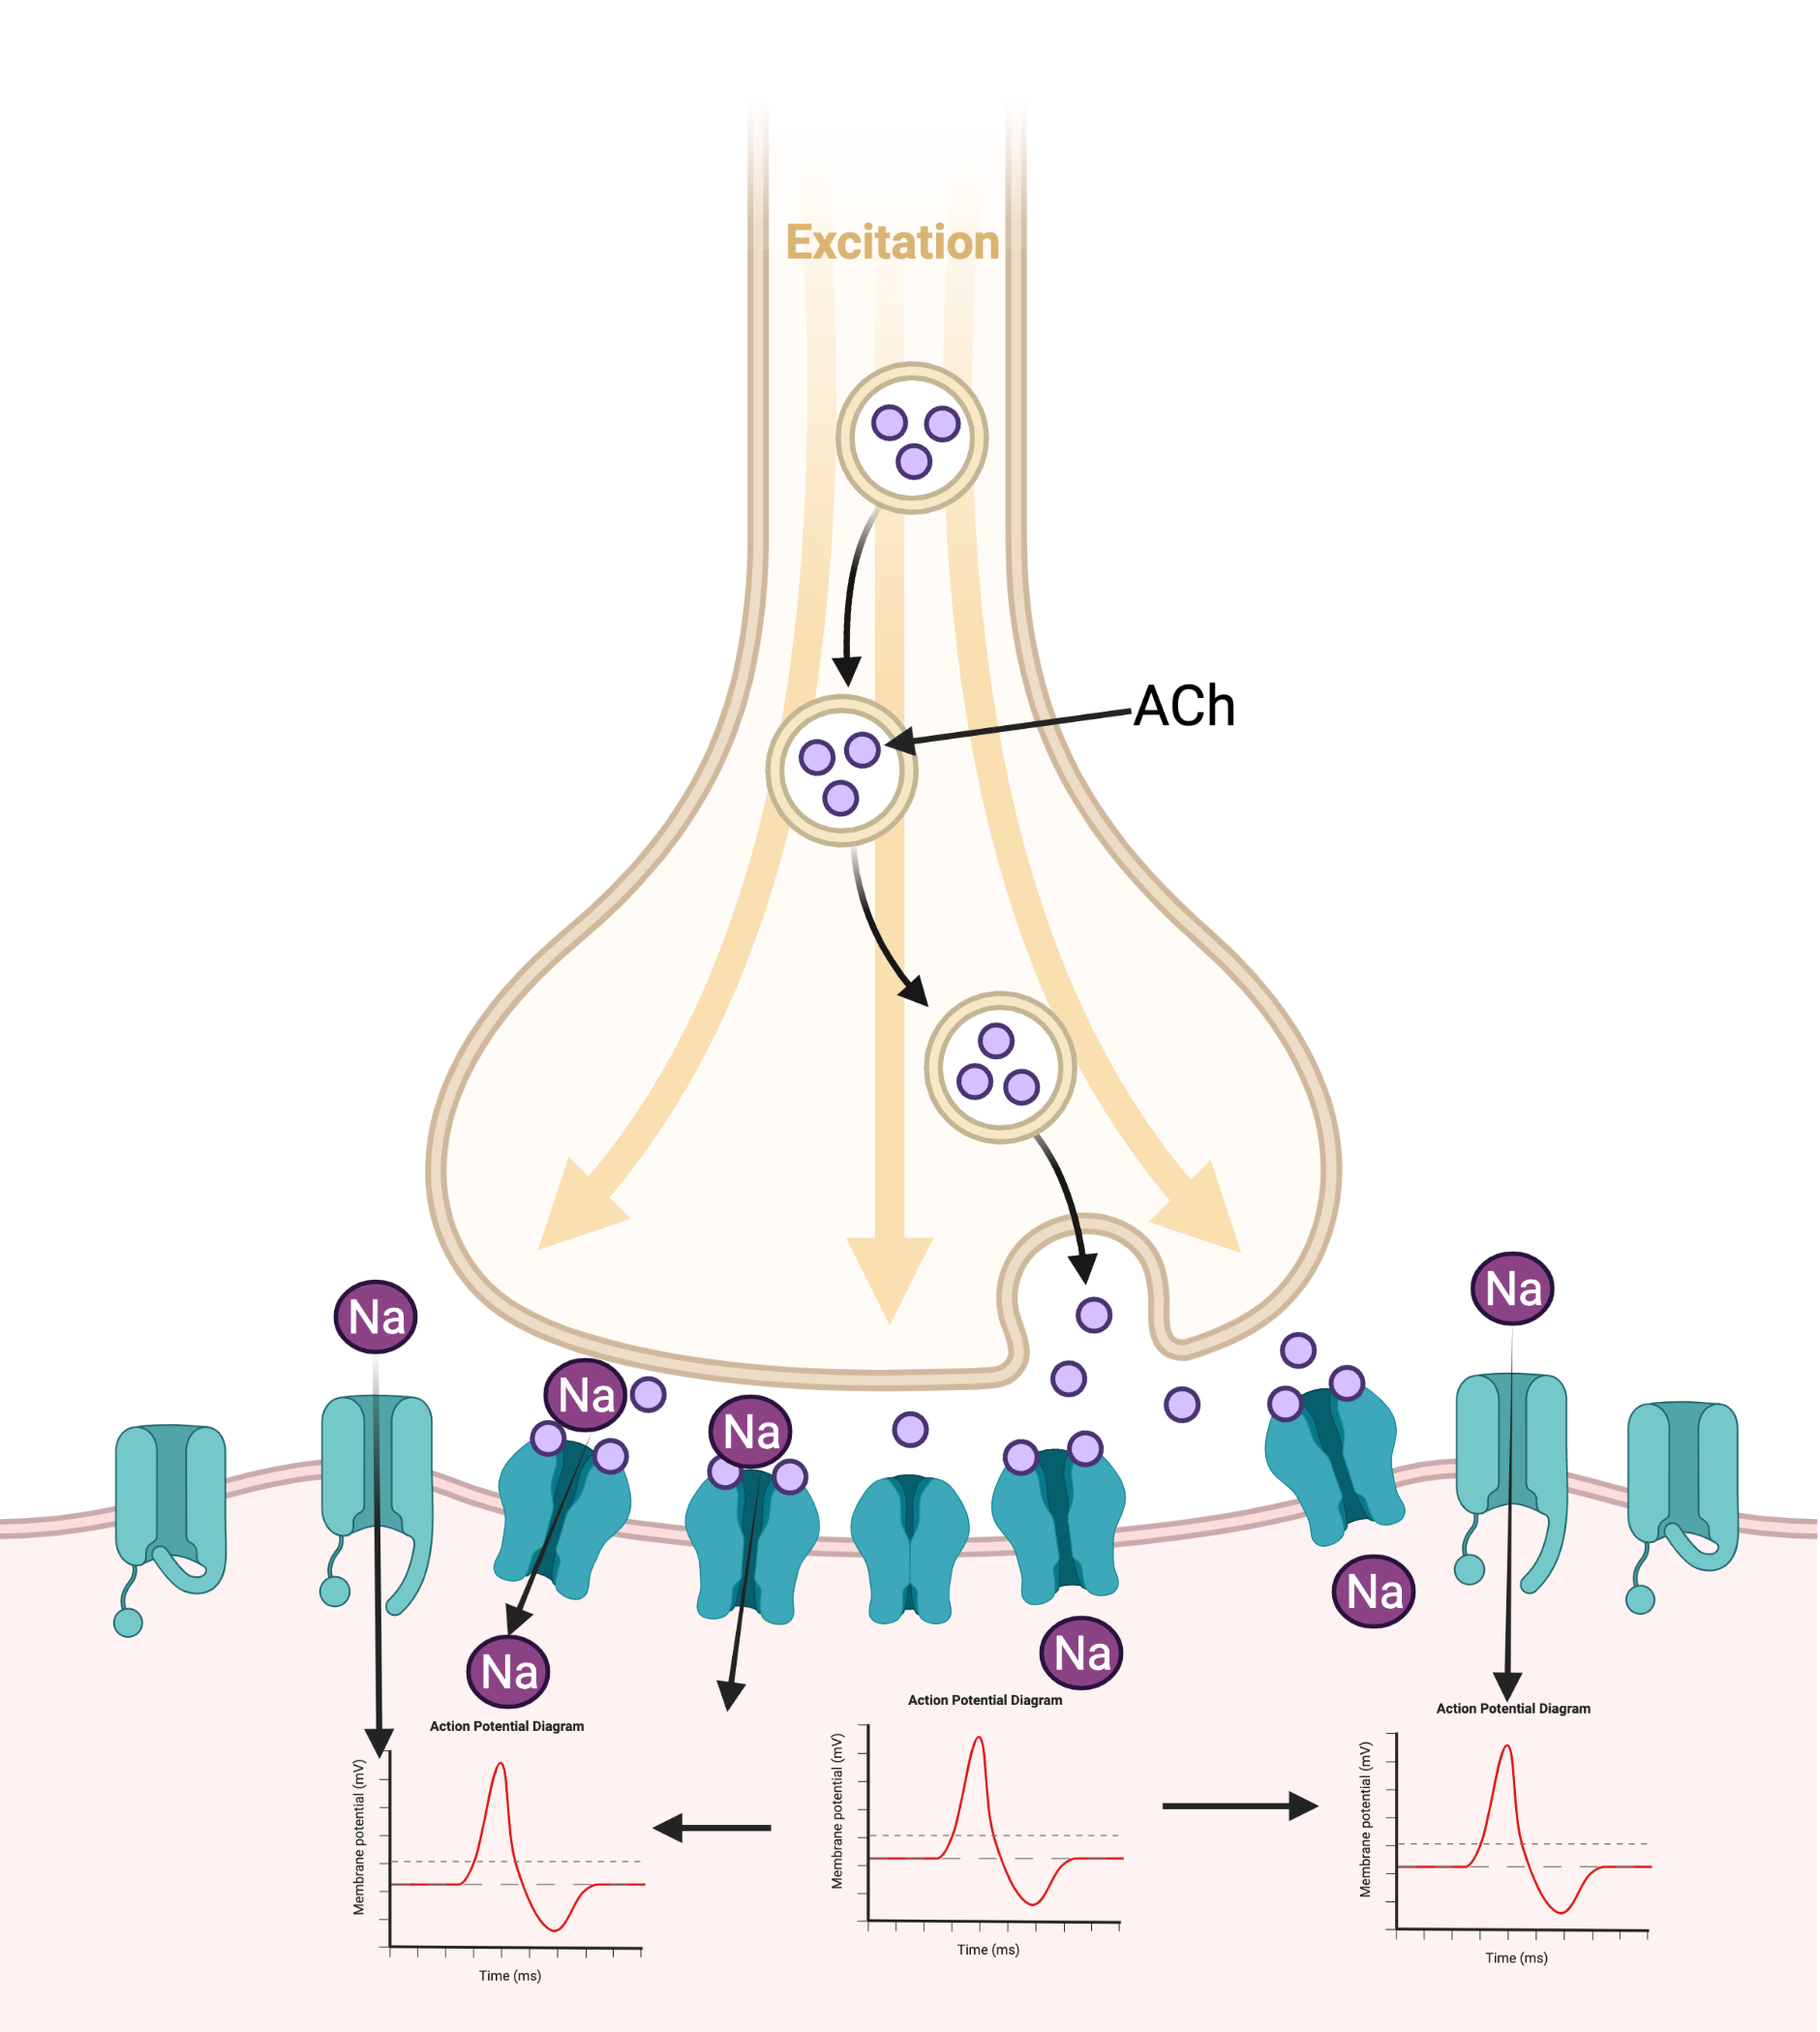
\includegraphics[width=1\linewidth]{./figure/NMJ.png}
    \caption{NMJ Excitation of the Motor End Plate \footnotesize{Created with BioRender.com}}
    \label{fig:NMJ}
\end{figure}

Excitation of the motor end plate spreads to the sarcolemma due to the opening of voltage gated ion channels on the sarcolemma. The sarcolemma excitation creates a wave similar to that in the axon (but without myelin) that spreads due to opening of voltage gated ion channels. The sarcolemma surrounds the fiber and penetrates the fiber and circles myofibrils through the intricate T-tubule system. T-tubules that encircle myofibrils form a triad with a SR on each side (See Figure \ref{fig:T-tubule}).

% Import the T-Tubule - SR triad image - CC from wikipedia

\subsection{Step 3 - Excitation - Activation Coupling (EAC)}
Excitation of the T-tubules excites the sarcoplasmic reticulum (SR). There are unique junctions between T tubules and the SR mediated by Ca channels. One acts as voltage sensors in the T tubules, and a second acts as Ca release channels in the SR.\footnotemark{}\footnotetext{The position of these two calcium channels differ between skeletal and cardiac muscle, which correlates with the functional differences in the control of contraction between these two types of muscle.} The implications of this unique T-tubule - SR junction is that excitation of the T-tubule quickly results in a combined excitation of the SR along with the release of Ca into the sarcoplasm\footnotemark\footnotetext{Sarcoplasm is the muscle fiber equivalent of the cytoplasm, the intracellular region that is in the cell but outside of any organelles (such as the SR, nucleus, mitochondria).} in close proximity of troponin binding sites for crossbridge activation (Figure \ref{fig:SR}).

% Figure of the sarcoplasmic reticulum - expand on Step 3?

\paragraph{Excitation \& EAC Latency}

Figure \ref{fig:eac-latency} represents each major phase of excitation and EAC from the $\alpha$-motor neuron to development of a twitch. The latency period is on the order of milliseconds (1/1000 of a second). The latency period of each excitation and EAC forms an upper boundary on the number of possible twitches per second. However, this boundary is determined by the latency of the excitation portion of Figure \ref{fig:eac-latency} which amounts to a few milliseconds. The fact that the twitch lasts for an estimated 100 ms means that excitation (a few milliseconds) can occur at a frequency that results in twitch (about 100 milliseconds) summation (add together to produce tetany).
\begin{figure}[!ht]
    \centering
    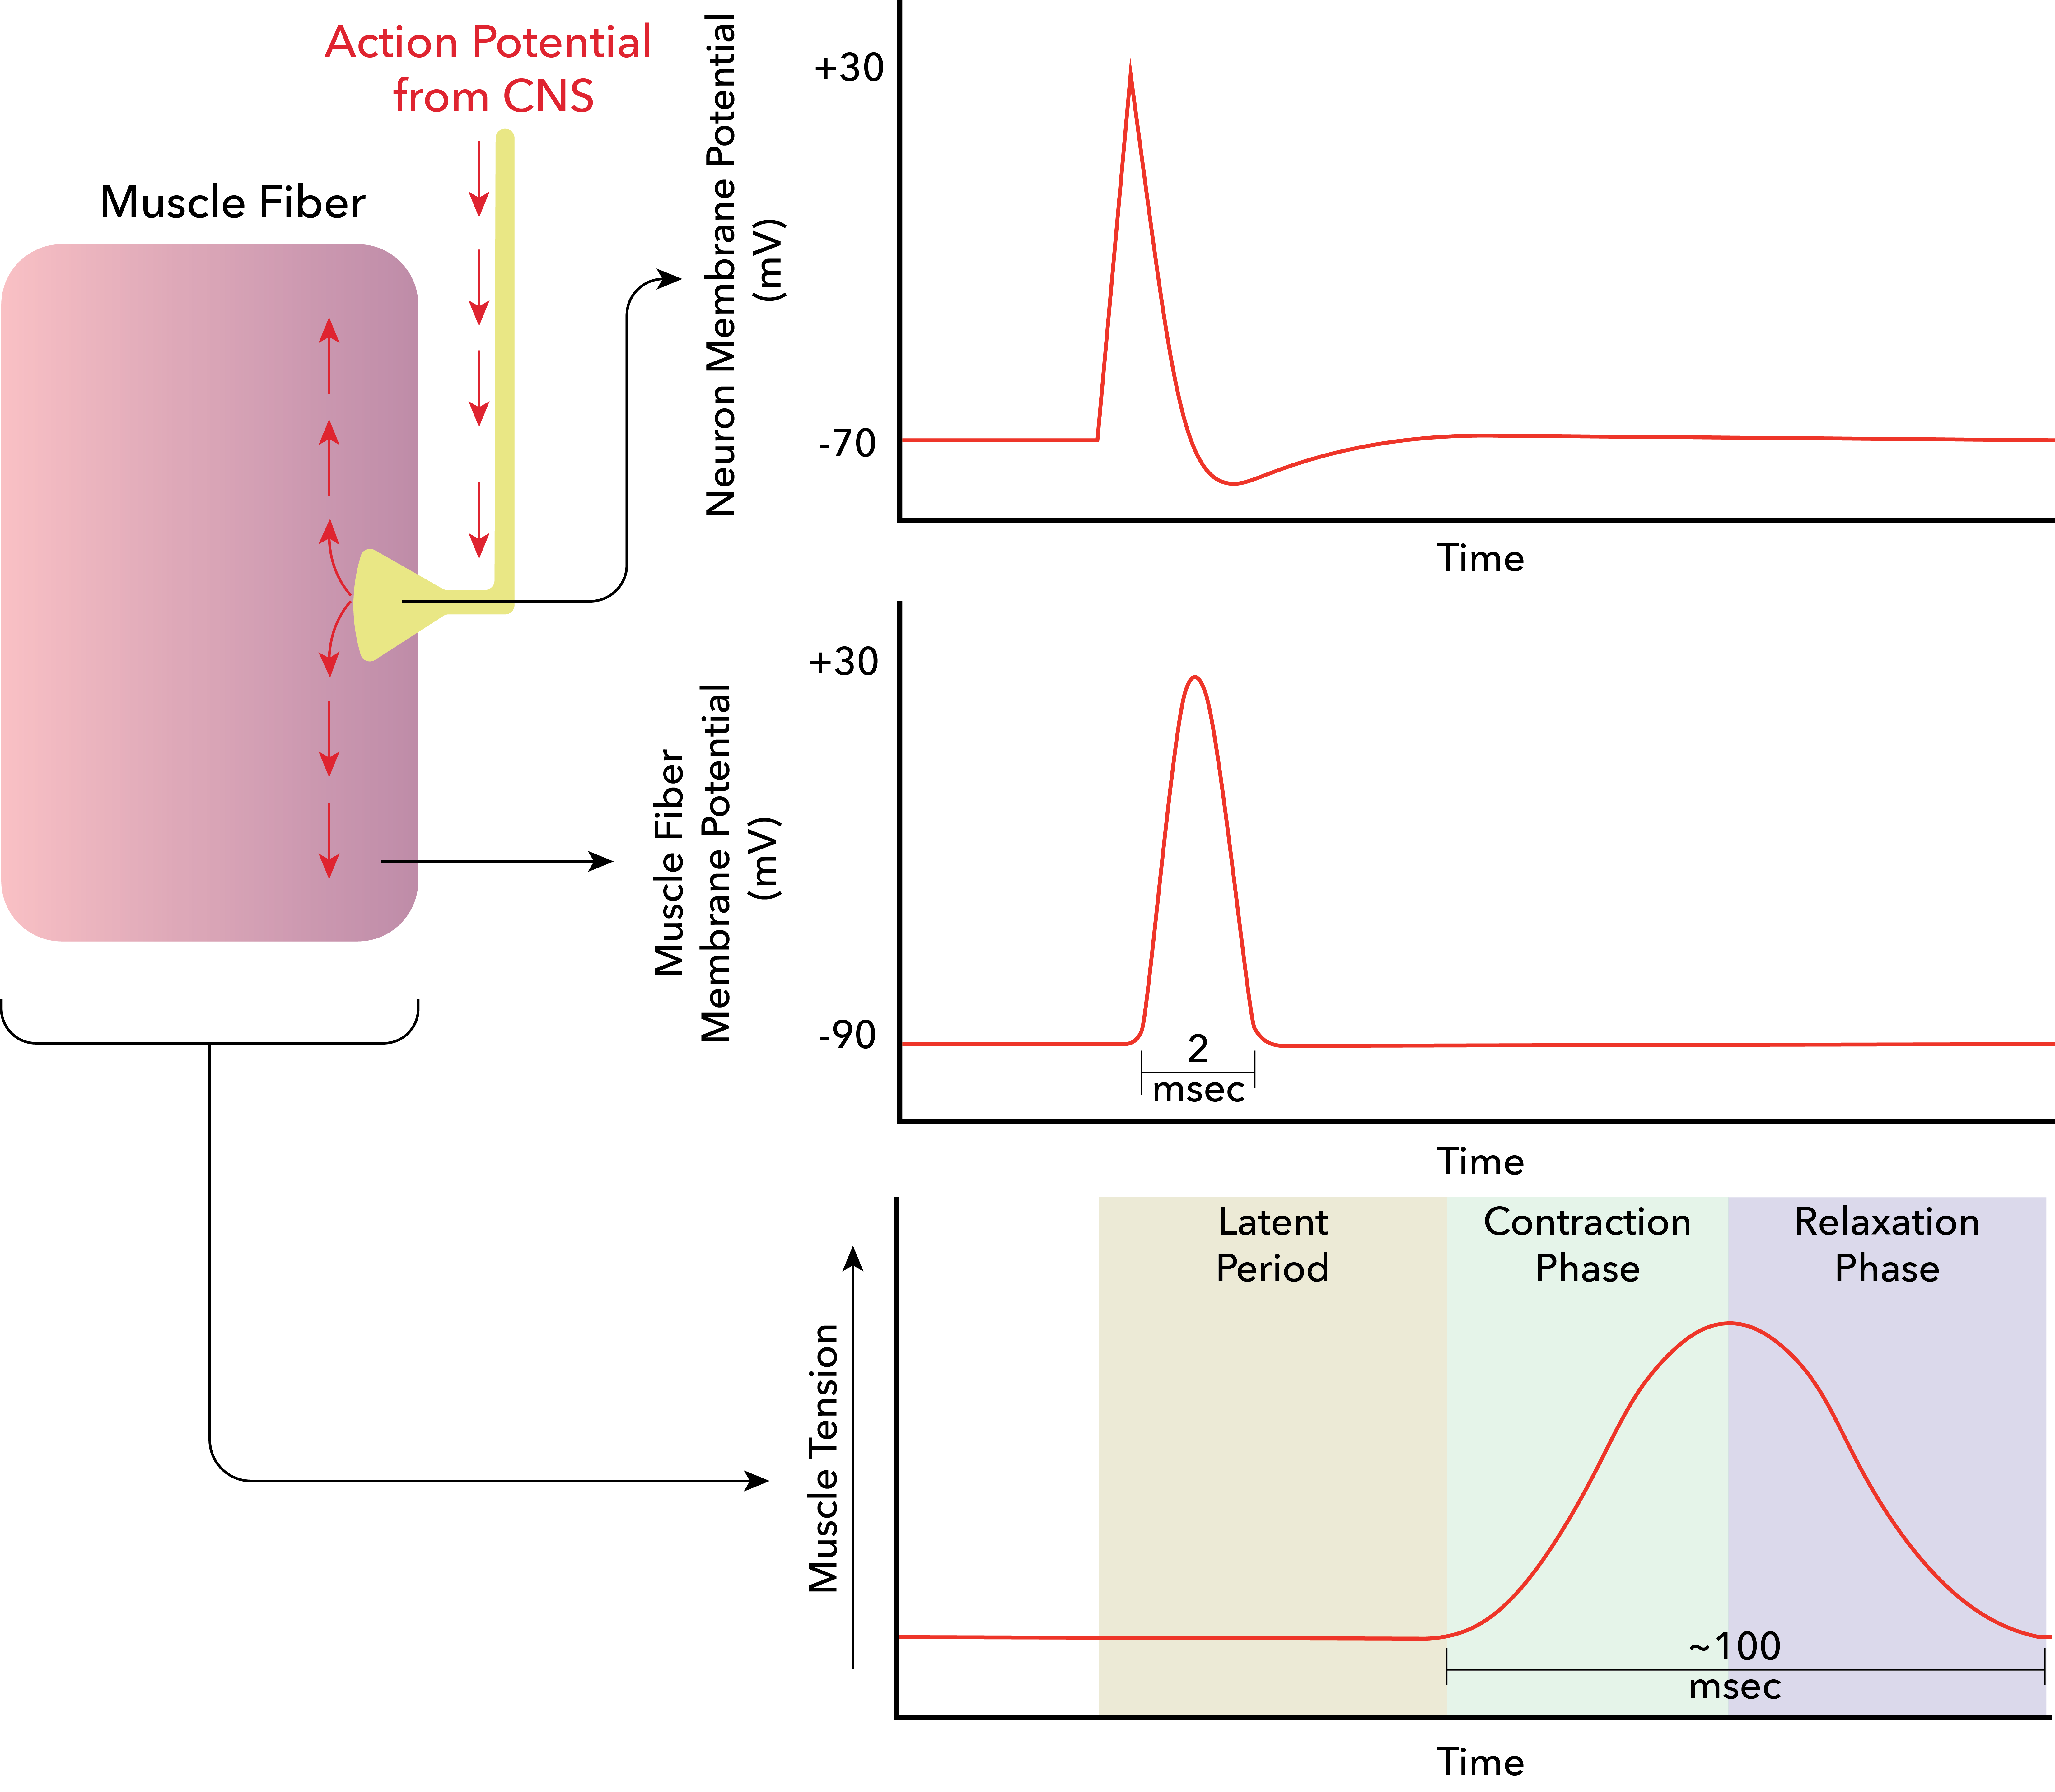
\includegraphics[width=1\linewidth]{./figure/eac-latency.png}
    \caption{EAC Latency \footnotesize{(Wikimedia Commons, CC BY 4.0, \href{https://commons.wikimedia.org/wiki/File:The_latent_period_between_the_muscle_action_potential_and_contraction.png}{EAC-Latency})}}
    \label{fig:Motoneuron}
\end{figure}

\subsubsection{Twitch to Tetany}
Each excitation activates enough crossbridges to produce a twitch. A twitch is the fundamental unit of active tension. However, a single twitch of active tension is not attaining tension when the goal of attaining tension is some sort of voluntary movement or stability. The rise and rate of a twitch depends on the amount and spread of Ca released, the available troponin sites, the available crossbridges to activate as well as the amount of elasticity in the series. One mechanism of muscle fatigue is a reduction in the release of Ca from the SR. The rate of Ca release from the SR can be increased in experimental preparations with caffeine. Low concentrations of caffeine bind to the voltage gated Ca channels at the junction of the T-tubule SR and increase Ca release during otherwise normal activation. However, high concentrations result in contracture without the need for the normal excitation signal. 

%A twitch can be an experimentally manipulated event. An electrical stimulus is provided to a muscle which results in either, or a combination of, $\alpha$-motor neuron excitation and sarcolemma excitation that excites the SR and activates enough crossbridges to produces enough active tension to produce a measurable force. A twitch can also be initiated by isolated (single) excitation of an $\alpha$-motor neuron, or isolated excitation of an $\alpha$-motor neuron or sarcolemma. 


\paragraph{Tetany}
Repeated excitation results in repeated activation and therefore continued crossbridge activation and repeated twitches (Figure \ref{fig:tetany}). Successive twitches create tension summation and is called tetany. When the force of active tension is measured, such as during a muscle test, it is the result of many muscle fibers being in tetany. The use of twitch frequency to create tetany and regulate active tension is detailed in Chapter \ref{chp:regulation}. 

%Add a figure of twitches becoming tetany

\subsubsection{Removal of Ca from Sarcoplasm}
Removal of Ca from the sarcoplasm requires active transport with Ca ATPase. This pump is dependent on Mg and moves 2 Ca into the SR while moving on H out at the cost of 1 ATP. Sarcoplasm levels of Ca can quickly return to resting levels which is necessary for rapid muscle relaxation and therefore muscle tension regulation and coordination. Situations that result in a delay in the removal of Ca from the sarcoplasm can delay muscle relaxation producing extra twitches or spasms (involuntary tetany). Since Ca ATPase is dependent on Mg, a deficiency in Mg can create such a situation.

\subsection{Return to Resting (Non excitation) State - RMP}
The process of returning to the resting state (RMP) is not explicitly discussed in the above sequence of membrane excitation events. It is implied, or taken for granted, once we started discussing the excitation of a twitch to the excitation of tetany (the summation of many twitches). Excitation of tetany requires that the axon, axon terminal, motor end plate, sarcolemma and T-tubule return to a resting (non excited) state. Notice, there is no excitation summation, only twitch summation.
\paragraph{}
Excitation occurs quickly because the resting state includes potential energy for excitation. The RMP is a polarized membrane with large ion concentration gradients (just waiting to run downhill with their gradients). This potential energy comes at a cost of spending energy (ATP) to pump ions against a concentration gradient. The RMP enables rapid excitation because ions are waiting with potential energy due to their concentration gradient to move quickly across the membrane (depolarize). 
\paragraph{}
The RMP also enables rapid return to the resting state with potential energy. The movement of K and Cl ions with their concentration gradient can quickly end excitation enabling the membrane to be quickly returned to RMP for another excitation. However the long term stability of the RMP relies on processes that depend on ion pumps to sustain concentration gradients for a lifetime.\footnotemark\footnotetext{Brain and heart death are situations where the cells of the brain and heart no longer return to the resting state, they no longer repolarize to the RMP, and therefore they can no longer undergo excitation.}
A deeper understanding of excitation and return to RMP, and clinical connections, requires a molecular and cellular understanding of excitable membranes.

%NEed to add Ca pumping back into the SR

% Stopped here - but need to add figures above.

\section{Excitable Membranes}

Membrane excitation (depolarization) requires the resting potential state (polarization). A membrane cannot depolarize unless it is first polarized. Additional detail about excitable membranes such as understanding of how the resting state is established, how this resting state is excited, and how this wave of excitation spreads, is necessary to understand muscle excitation and how various clinical situations may influence excitation.

% Moved from above - not sure what to do with this....
Signal transmission that results in cellular events (including along the membrane) it is called signal transduction. The action potential signal transduction that occurs along the surface of a nerve and muscle membrane is facilitated by the presence of voltage gated channels embedded in the membrane. Signal transduction from a membrane to another membrane is facilitated by ligand gated channels at specific places in membrane. The detailed physiology of excitable membranes such as establishing and maintaining a resting membrane potential, and mechanisms that result in action potentials are important details covered later in the chapter. 
%------------------

\subsection{Excitable Membranes}

Excitable membranes have the capability of being in two states, a resting state and an excited state. The difference between these states is the electrical potential across the membrane. In the resting state the membrane is said to be polarized. In the excited state the membrane is not polarized, more commonly referred to as depolarized. The resting membrane potential (RMP) is a particular polarized potential across the membrane and includes the inside of the cell (intracellular) being more negative than the outside of the cell (extra cellular). By convention this is considered negative polarity.\footnotemark{}\footnotetext{This is by convention because it is a choice to describe polarity relative to the intracellular space. If we choose to describe polarity relative to the extra cellular space then the polarity is positive} During excitation an action potential (AP) changes the membrane potential (MP) from negative polarity to positive polarity for a short period of time (how long the MP has positive polarity depends on the particular cell membrane).

The RMP is not a natural (physically neutral) state. We consistently expend energy to maintain the RMP against a natural tendency for the polarity to dissipate. It is helpful to understand the cell membrane before further discussion of the events that establish RMP and allow for an AP.

\subsubsection{Cell Membrane}

The cell membrane is a semipermeable phospholipid bilayer barrier that forms a boundary for the cell. Part of its semipermeability is related to combination of the bilayer being hydrophobic (detracts water) and the inside of the membrane being hydrophilic (attracts water) which limits what can freely diffuse through the membrane. And part is due to the particular transport proteins within the membrane for selective forms of active, facilitated and passive transport. The membrane separates the intracellular from the extra cellular space. Through selective transport it establishes the conditions for cellular activities within the cell and thus influences (but does not completely establish) conditions outside the cell. Cell membranes are dynamic structures that adapt in response to the intracellular and extra cellular conditions to meet the needs of the cell.

Figure of a cell membrane

\paragraph{Sodium Potassium ATPase Pumps}
$Na^+/K^+$ ATPase pumps are embedded throughout excitable membranes. These protein based molecular machines convert the energy of ATP to the movement of three $Na^+$ outside the cell and two $K^+$ inside the cell with each cycle of the pump (each use of ATP). Given the natural tendency of molecules to move based on a concentration gradient (high concentration to low concentration) the resultant higher concentration of  $Na^+$ outside and higher concentration of $K^+$ inside the cell requires the work of these active transport pumps against the concentration gradient.

Figure of pumps

Refer to figure of the cell membrane 

\paragraph{Channels \& Receptors}
Channels are proteins embedded in the cell membrane that allow passage of molecules between the intracellular and extra cellular space. Channels can be gated and therefore only allow passage under certain circumstances. 
Voltage gated channels only allow passage when the membrane potential is at certain values. They may open at a certain value and close a certain period of time later; or they may close at a certain value and open a period of time later. 
Ligand gated channels only allow passage when the channel is activated due to the binding of a ligand (a molecule that can bind). A ligand gated channel is also a receptor, or closely associated with a receptor. 
Receptors are proteins that can bind to a ligand. Some receptors are ligand gated channels (a receptor where the activity that binding produces is opening a channel gate). Other receptors perform different activities within the cell. 

Figure of receptors

\paragraph{$Na^+$ \& $K^+$ Channels}

$Na^+$ channels allow the passage of $Na^+$ with its concentration gradient and can be either ligand gated or voltage gated. $K^+$ channels allow the passage of $K^+$ with its concentration gradient and in nerve and muscle excitable membranes are voltage gated. 

Refer to figure of the cell membrane

\subsection{Establishing the Resting Membrane Potential}

In a resting (non excited) state these membranes have a resting membrane potential (RMP). The RMP is a difference in electrical polarity across the membrane. For both nerve and muscle membranes the resting polarity is negative inside the cell relative to outside the cell. 


The resting membrane potential is an equilibrium potential. It is the consequence of two physiological situations. First, the presence of large concentration gradients for $K^+$ and $Na^+$ across the plasma membrane. Second, the relative permeability of the membrane to those ions. The concentration gradients for $K^+$ and $Na^+$ are the product of the activity of the $Na^+$-$K^+$-ATPase pumps. The concentration gradient maintains a large outwardly directed $K^+$ gradient, and the large inwardly directed $Na^+$ gradient.

The relative permeability of the plasma membrane to $Na^+$ and $K^+$ reflects the open versus closed status of ion-selective membrane channels. Different membranes display different degrees of permeability to different ions. In resting conditions the membrane of nerve and muscle cells are more permeable to $K^+$. Due to the concentration gradient $K^+$ flows out of the cell. As if flows out it creates a negative potential (leaves behind net negative charge inside the cell). However, this negative potential also works to prevent the flow of $K^+$ outside of the cell. The negative potential inside the cell attracts positive ions. Since the $K^+$ is the positive ion what the cell membrane is most permeable the outward flow of $K^+$ due to the concentration gradient is decreases to no net flow of $K^+$ due to the electrically driven inward flow (pull, attraction) for $K^+$ as a positive ion by the negative potential inside the cell. The potential that this balance between outward flow of $K^+$ due to concentration, and inward flow of $K^+$ due to electric potential is called the equilibrium potential. The resting membrane potential is the equilibrium potential. Since $K^+$ has the highest permeability at rest, the resting membrane potential is primarily influenced by the equilibrium potential of $K^+$.

Under normal, healthy, conditions different cell membranes have slightly different resting membrane (equilibrium) potentials. These differences are due to differences in the permeability of the membranes to $K^+$ (or to other ions, such as $Na^+$, $Cl^-$, $Ca^{2+}$). The extra cellular concentration of these ions is held constant throughout the body and therefore under normal circumstances differences in the concentration gradients are not a major source of differences in resting membrane potentials. 


\subsection{Trigger \& Spread of Sarcolemma Excitation (AP)}

An action potential involves the opening of voltage gated $Na^+$ channels due to a change in voltage in the resting membrane potential (becoming less negative). The number of voltage gated $Na^+$ channels that open is proportional to the change in the membrane potential. This cycle of opening in response to a voltage change is self perpetuating since once a $Na^+$ channel opens $Na^+$ flows into the cell due to the $Na^+$ concentration gradient. Due to the movement (not a change in the actual gradient) the membrane potential voltage changes (becomes less negative). The point that approximately half of the voltage gated $Na^+$ channels open is considered a threshold potential. At the threshold potential the voltage gated $Na^+$ channels continue to rapidly open until the equilibrium potential approaches that of $Na^+$ (as opposed to $K^+$) since at this point the membrane is more permeable to $Na^+$. The equilibrium potential for $Na^+$ is approximately 65 mV.  Once a membrane reaches the threshold potential an action potential is said to have occurred. It is at this point that the action potential is said to be “all or none.” Either it occurs or it does not occur. Prior to the threshold potential membranes can undergo micro potential changes. These micro potentials can be depolarizing (excitatory potentials that move the membrane potential toward the threshold), or hyperpolarizing (inhibitory potentials that move the membrane potential further away from the threshold potential).

Voltage gated $Na^+$ channels have two gates. One is an activation gate and it is closed under resting conditions and opens during excitation. The second is an inactivation gate and it is open under resting conditions but closes soon after the activation opens. The inactivation gate closure is timed, it is not triggered by events outside of the molecule itself. The inactivation gate is the first step to stopping an action potential. At this point the activation gate is open and the inactivation gate is closed. To be reset and completely ready for another action potential the activation gate must close and the inactivation gate must open (these are timed events). After an action potential the period of time that a large proportion of the $Na^+$ gates not yet reset is called the \textbf{absolute refractory period}. It is the period that regardless of how large a stimulus, the membrane cannot undergo another action potential. 

%%% Need to look up the timing of these events and relate to refractory periods….

Voltage gated $K^+$ channels open but are delayed when compared to $Na^+$. When they open the permeability for $K^+$ increases and the outward flow of more $K^+$ than under resting conditions starts to return the membrane potential to its resting value. Therefore, the opening of the $K^+$ channels is the second step to stopping an action potential. A short time after opening the $K^+$ will close (also a timed event, not triggered by outside events). During the time that the $Na^+$ gates are reset and the $K^+$ gate remains opened the membrane is said to be in a \textbf{relative refractory period}. It is the period that a normal stimulus the membrane will not achieve an action potential, but with a larger than normal stimulus an action potential is possible. 

Spread of excitation occurs because when one area of a membrane depolarizes during an action potential the change in membrane potential at nearby sections of the membrane starts the self perpetuating process of opening voltage gated $Na^+$ channels. This spread occurs in one direction (meaning it does not result in cyclic repeating action potentials of the entire membrane) because of the refractory periods. If a membrane is visualized as a set of dominoes and the resting potential is when the dominoes are upright, and an action potential is when a domino falls, then the refractory period is the period when the domino is still fallen. Because of the fallen domino on one side of the next falling domino, the dominos fall in one direction away from the starting stimulus. (Section needs work - and a figure)

\section{$\alpha$-motor Neuron Excitation \& the Neuromuscular Junction}

The beginning of muscle fiber excitation is motor end plate excitation. The motor end plate is a specialized are of the sarcolemma that has receptors, specifically ACh receptors that are also ligand gated $Na^+$ channels. These ligand gated $Na^+$ channels open when ACh binds to them which changes the membrane potential of the motor end plate. If there are just a few ACh receptor gates open then there may be an excitatory potential (also called a excitatory post synaptic potential (EPSP) since at this point the motor end plate is after (post) the synapse from the $\alpha$-motor neuron). However, if enough ACh receptor gates open and the voltage changes enough to open voltage gated channels, and the membrane potential reaches its threshold value then an action potential will occur in the motor end plate. This excitation will then spread along the entire sarcolemma down to the the T-tubules, resulting in the release of $Ca^{2+}$ from the SR. $Ca^{2+}$ in the muscle fiber will change the state of crossbridges from inactive to active. This single excitation may produce a twitch (a measurable generation of force from active tension) as long as the $Ca^{2+}$ released results in enough active crossbridges. 

\paragraph{Excitation to Regulation}

Many events have just been described for one excitation, particularly since one excitation is hardly enough to create a twitch, and a twitch is not enough to produce meaningful movement. A more efficient system of excitation-activation coupling exists in the cardiac muscle. However, in the skeletal muscle the efficiency of creating tetany from one excitation is sacrificed for the sake of regulation of muscle tension. Since creating tetany requires many action potentials, then the amount of tetany can be regulated by the number of action potentials. The regulation of muscle fibers is the topic for Chapter \ref{chp:regulation}.


Add Chloride channels and their RMP stabilizing role

\section{\textit{Clinical Physiology Connections}}

The concepts of excitable membranes, receptors, ligand channels and signal transduction are pervasive throughout clinical physiology. In this final section of the chapter the connection is made between these topics to neuroendocrine, sensory receptors and pharmacodynamics.

\subsection{Neuroendocrine}

The neuroendocrine system regulates several critical physiological systems and coordinates cellular functions throughout the body. Examples include mobilizing the body for fight or flight reactions by getting all cells in the body ready to meet demands that require energy mobilization at the expense of other maintanence activities. For example, release of hormones for fight or flight will signal liver cells to hold off on using energy to repair the cell membrane and instead use energy to convert glycogen (a stored fuel) into glucose (a usable fuel). Amazingly the neuroendocrine system can alert cells all over the body to do activities that each of those cells can do for the fight or flight situation, even though those activities are varied between the cells. While the liver cells are releasing glucose, the heart cells are prepared to use more glucose and are working more frequently (higher rate) and harder (more pressure). The differentiation of tasks completed by these cells is due to the specialization of the cells, and due to the receptors around the body that are responding to the same ligand. Most cells in teh body have a ligand receptor for epinephrine (a major catecholamine of the fight or flight response). Epinephrine is also called adrenaline. Receptors for epinephrine are therefore called adrenergic receptors. The adrendergic receptors on all cells have a similar binding location for epinephrine, but the receptor itself transducts different signals into the cell depending on the receptor and depending on the cell. 

\subsection{Sensory Receptors}

Sensory receptors are specialized receptors at the terminal end of the axon of a sensory neuron. They differ from ligand and voltage gated receptors in the signals that provokes their excitation. In general, the signal the provokes excitation in a sensory neuron is whatever phenomenon or sensation that sensory neuron is associated. If the sensory neuron is excited by changes in temperature then it is a temperature sensory neuron; if by changes in tension, it is a tension sensory receptor; if by vibrations, it is a vibration (as in the ear) sensory receptor; if by photons, it is a light sensory receptor (as in the retina); if by certain non specifically chemicals or ions (such as hydrogen for pH) they are chemoreceptors; if by changes in pressure they are baroreceptors. Some sensory receptors terminate in areas of the brain that allow perceptions of the signal in a way that gives them additional meaning. For example, some chemoreceptors proceed to the brain and produce pain signals, once in the brain a complicated cascade of connections are made that can, over time, change from being protective to themselves harmful to movement. Other chemoreceptors that detect an increase in carbon dioxide proceed to areas in the nervous system to produce unconscious reflex responses (changing respiratory rate) and also to the brain (a general state of anxiety and air hunger). Some receptors don’t go to the brain at all, but interact at areas in the nervous  system where responses are automatic (baroreceptors as part of the autonomic nervous system to regulate blood pressure). Since baroreceptors don’t go to the brain at all we do not perceive what our blood pressure is directly - making elevated blood pressure a “silent killer.” Most physiological  homeostasis regulatory networks involve a sensory receptor of some type that contributes to the monitoring of a homeostatic variable. 

\subsubsection{Sensory Receptor Dynamics}
As receptors the sensory receptors (all of them) are subjects to the same dynamics discussed as part of the cell membrane and pharmacodynamics. When a sensory receptor undergoes up regulation or down regulation there are then changes to when the sensory receptors signal their respective neurons. With upregulation of chemoreceptors for carbon dioxide an individual will tend to have a higher respiratory rate and maintain a lower carbon dioxide level since their response to carbon dioxide is increased. The upregulation then continues to propagate itself. Since it results in lower carbon dioxide levels, the receptors remain upregulated in an attempt to be able to respond to lower carbon dioxide levels. A balance point is eventually achieved. But this new balance point may be enough to result in what is converted altered homeostasis.

\subsubsection{Neuromuscular Sensory Receptors} 
There are several important neuromuscular sensory receptors that sense signals from the muscle, musculotendonous junction and/or the tendon. Signals for tension (such as golgi tendon organs), signals for changes in length (such as the muscle spindle), and signals for the chemical constituents of the extra cellular fluid surrounding muscle fibers (chemoreceptors). These receptors and their role in muscle function will be covered in upcoming chapters on regulation, energetics and micro-circulation.

\subsection{Pharmacodynamics}

Pharmacodynamics considers the biochemical and physiologic effects of drugs. The biochemical effects are completely related to the drug as a ligand. 

\section{Summary \& Next Steps}


% Figures

\begin{figure}[!ht]
    \centering
    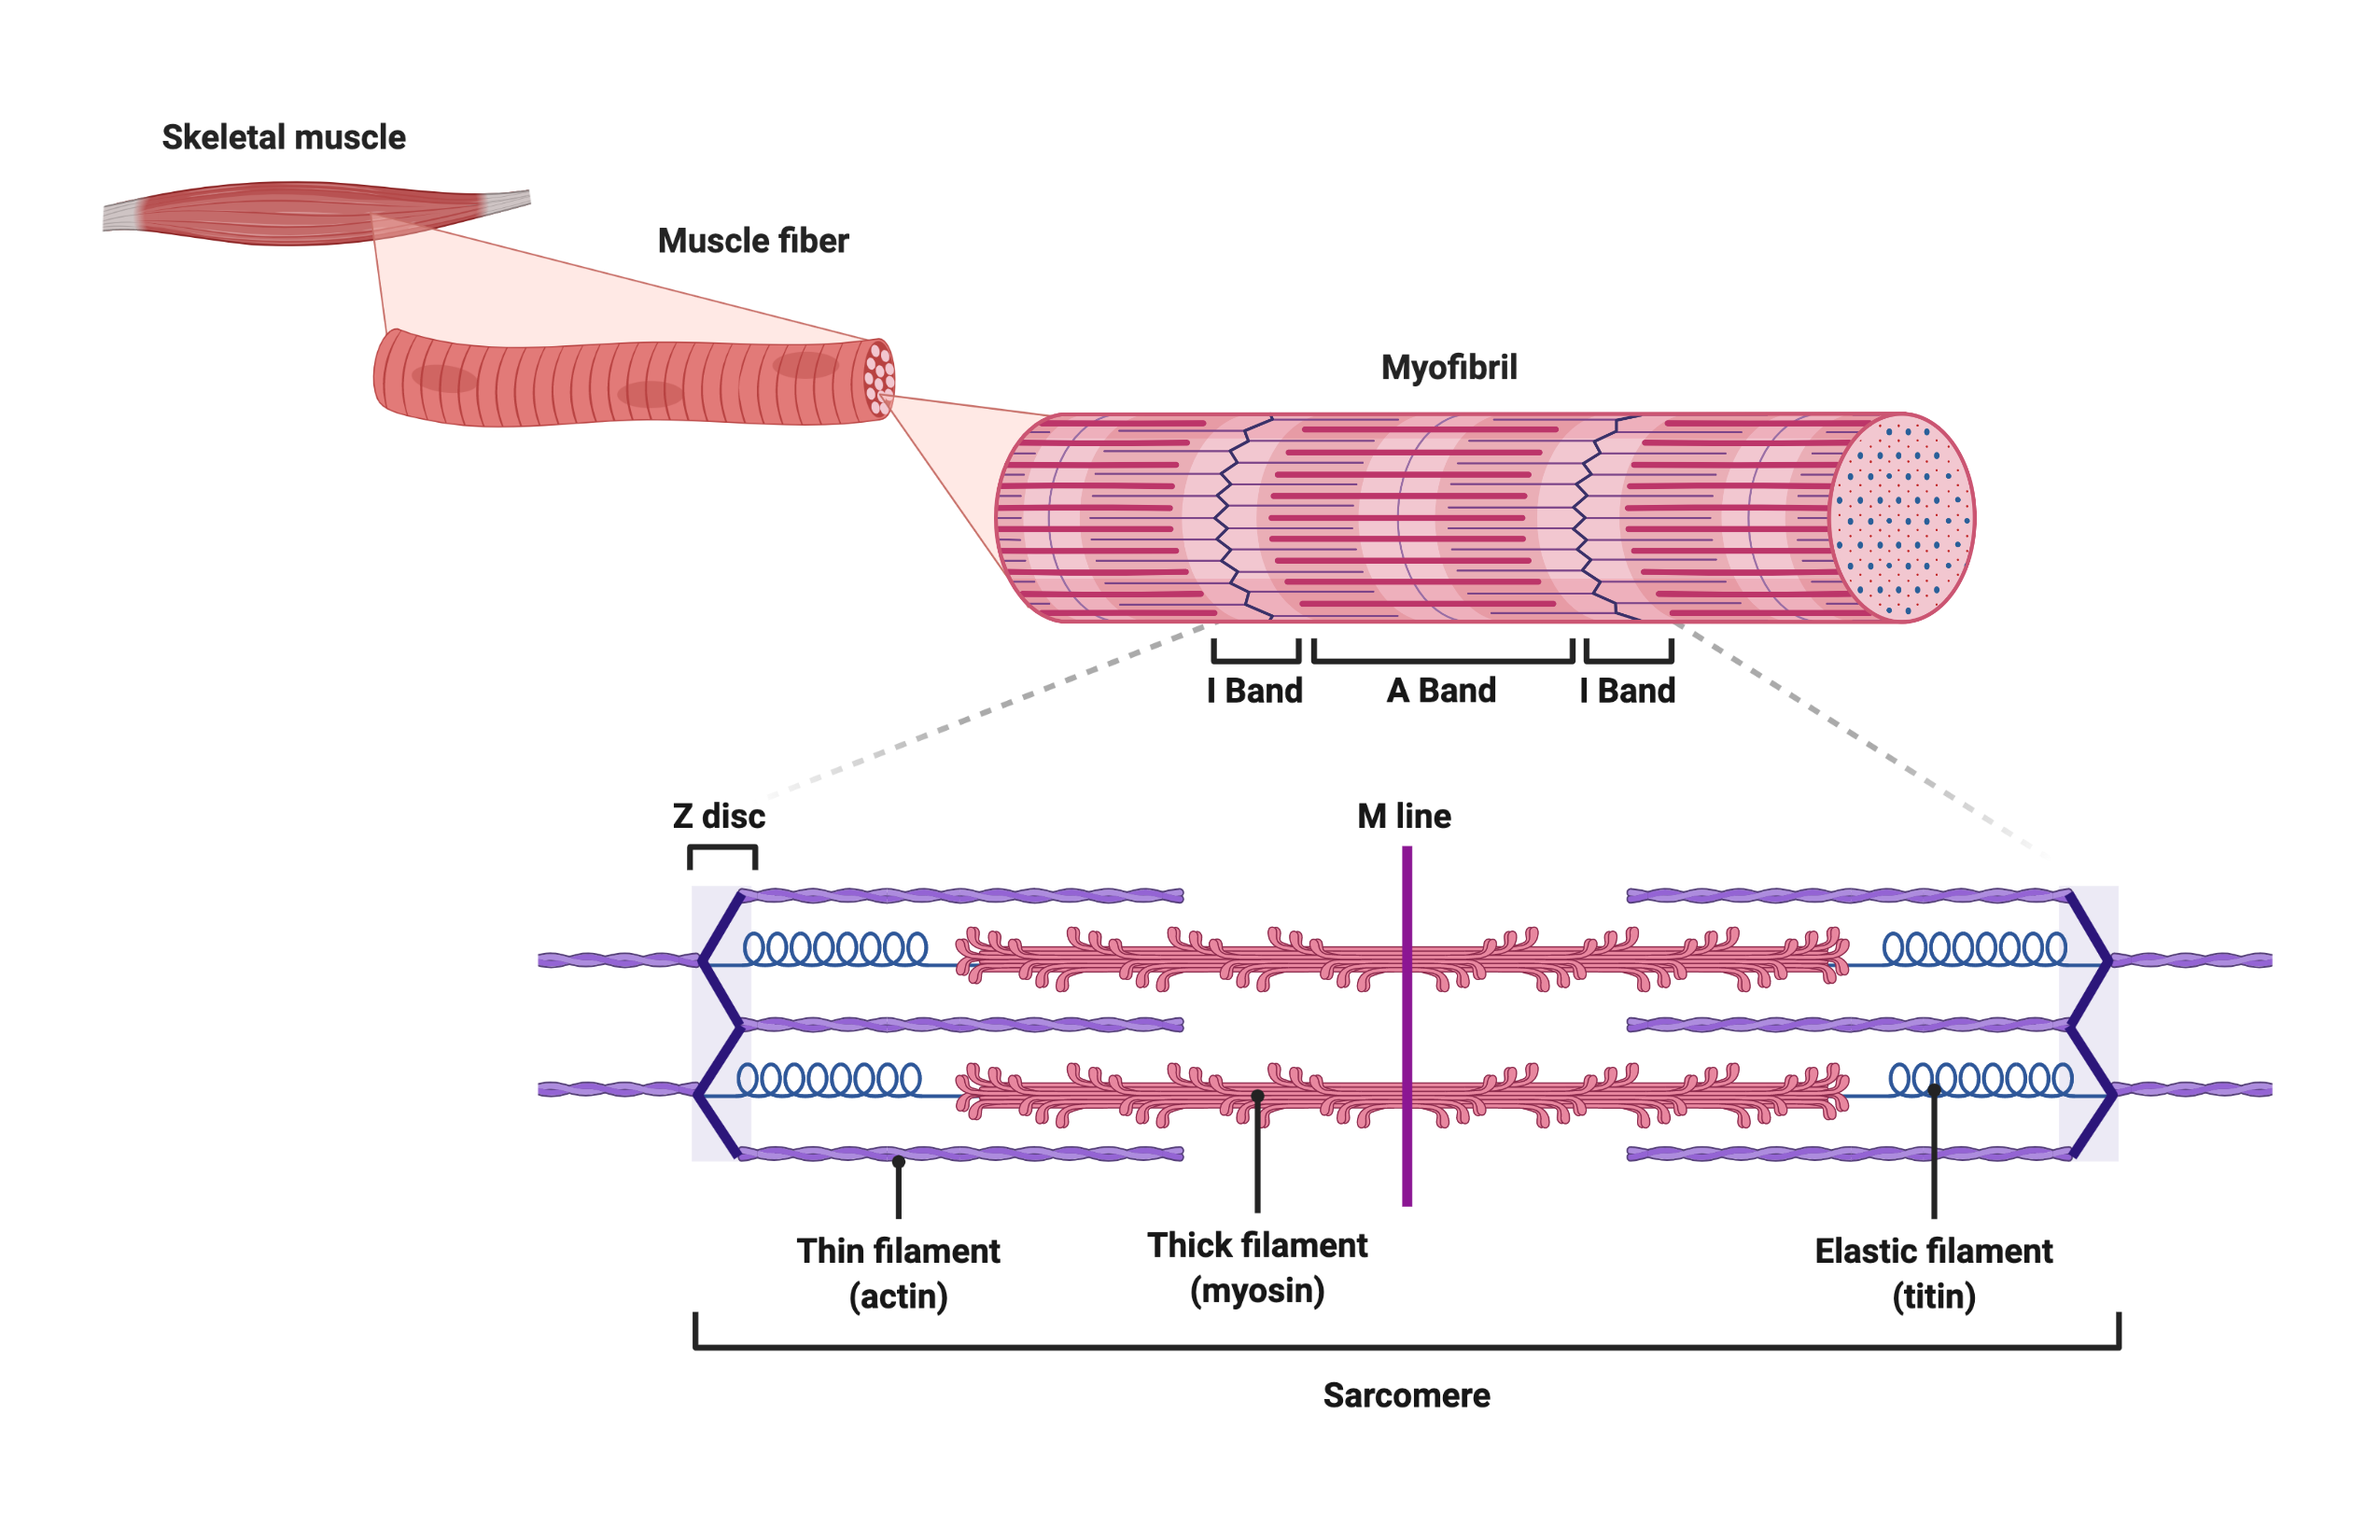
\includegraphics[width=1\linewidth]{./figure/Myofibril_Structure.png}
    \caption{Myofibril Structure \footnotesize{(Created with Biorender.com)}}
    \label{fig:Myofibril_Structure}
\end{figure}


\begin{figure}[!ht]
    \centering
    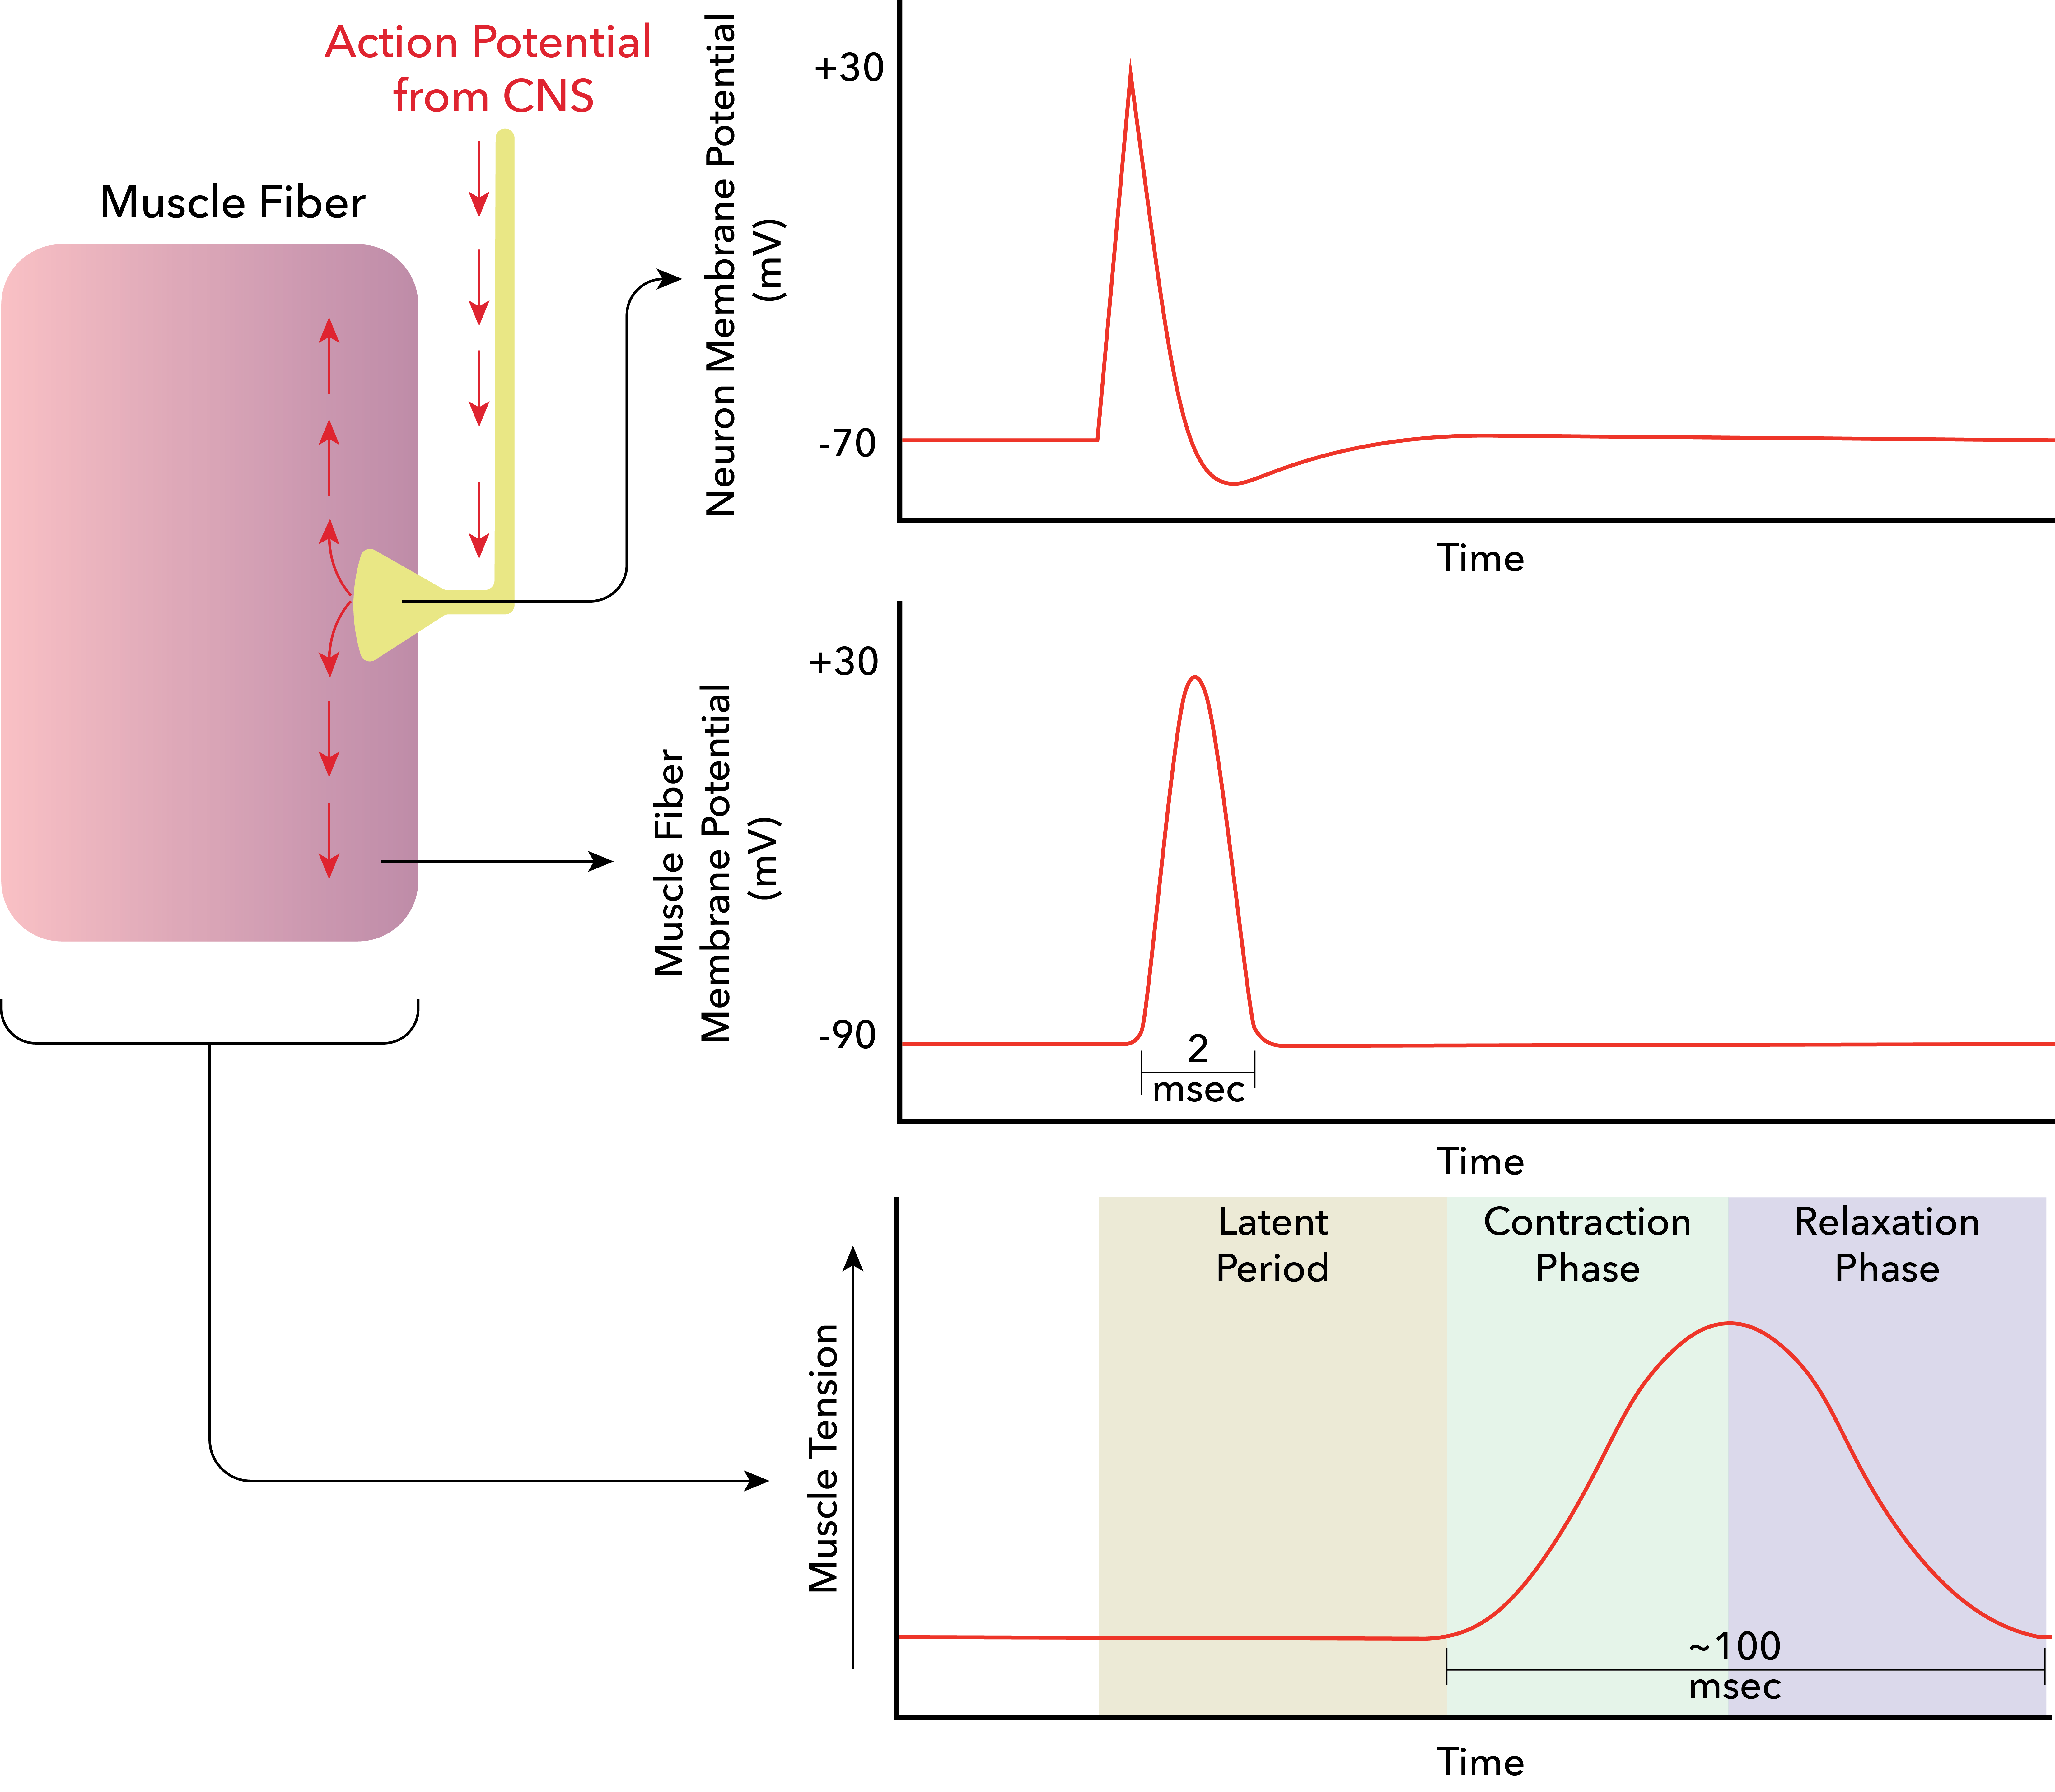
\includegraphics[width=1\linewidth]{./figure/eac-latency.png}
    \caption{$\alpha$-motor neuron terminating at several muscle fiber motor end plates \footnotesize{(Wikimedia Commons, CC BY 4.0, \href{https://commons.wikimedia.org/wiki/File:Motoneuron.png}{Motoneuron})}}
    \label{fig:Motoneuron}
\end{figure}

\printbibliography[heading=subbibintoc]



